\documentclass[11pt,a4paper,twoside]{article}

\usepackage[utf8]{inputenc}
\usepackage[T1]{fontenc}
\usepackage[english]{babel}
\usepackage{graphicx}
\usepackage{latexsym,amsmath,amssymb,amsthm}
\usepackage{makeidx}
\usepackage[usenames,dvipsnames]{color}
\usepackage[unicode=true,colorlinks=true,linkcolor=RoyalBlue,citecolor=RoyalBlue]{hyperref}
\usepackage{natbib}
\usepackage{lipsum}
\usepackage{hyperref}

% C++ formatting
\usepackage{listings}  % for code formatting
\usepackage{color}
\definecolor{listinggray}{gray}{0.9}
\definecolor{lbcolor}{rgb}{0.9,0.9,0.9}
\lstset{
  backgroundcolor=\color{lbcolor},
  tabsize=4,
  language=C++,
  captionpos=b,
  tabsize=3,
  frame=lines,
  numbers=left,
  numberstyle=\tiny,
  numbersep=5pt,
  breaklines=true,
  showstringspaces=false,
  basicstyle=\footnotesize,
  identifierstyle=\color{magenta},
  keywordstyle=\color[rgb]{0,0,1},
  commentstyle=\color{OliveGreen},
  stringstyle=\color{red}
}


\title{The Feed Forward Neural Network library}
\author{Francesco Calcavecchia}

\makeindex

\newcommand{\MRTWO}{$ \text{M}(\text{RT})^2 \;$}
\newcommand{\actf}{\text{a}_f}
\newcommand{\logaf}{\sigma_{\text{lgs}}}
\newcommand{\tansaf}{\sigma_{\text{tans}}}
\newcommand{\gssaf}{\sigma_{\text{gss}}}
\newcommand{\sinaf}{\sigma_{\text{sin}}}
\newcommand{\idaf}{\sigma_{\text{id}}}
\newcommand{\reluaf}{\sigma_{\text{ReLU}}}
\newcommand{\seluaf}{\sigma_{\text{SELU}}}


\begin{document}
\maketitle

FFNN (Feed Forward Neural Network) is a C++ library which allows the implementation of a feed forward neural network with few simple calls.
The library includes a training method, which currently utilizes GSL nonlinear
multifit routines (trust region based Levenberg-Marquardt) to achieve least
square fitting against target data. A data split into training, validation and
testing is supported and enables early stopping. The library features inherent data
normalization, completely hidden from the user.
In terms of derivatives of the NN value, the library currently supports its
first and second derivatives with respect to the NN input, the first derivative with
respect to the variational weights within the FFNN and first/second order cross
derivatives, with respect to both input (first / second order) and variational
parameters (only first order).

The code has been developed using the standard C++11.

In the following we will present some classes made available by the library.
At the beginning we will report the necessary \verb+#include+ call and the
prototype of the class (not necessarily equal to actual code).

\section{FeedForwardNeuralNetwork}
\label{sec:feedforwardneuralnetwork}

\begin{lstlisting}
// #include "FeedForwardNeuralNetwork.hpp"
class FeedForwardNeuralNetwork
{
    // Constructor and destructor
    FeedForwardNeuralNetwork(const int &insize,
         const int &hidlaysize,
         const int &outsize);
    FeedForwardNeuralNetwork(const char * filename);
    ~FeedForwardNeuralNetwork();

    // Getters for the basic information
    int getNHiddenLayers();
    int getNLayers();
    int getLayerSize(const int &li);
    ActivationFunctionInterface *
         getLayerActivationFunction(const int &li);

    // Getters for the variational parameters
    int getNBeta();
    double getBeta(const int &ib);
    void setBeta(const int &ib, const double &beta);

    // Set the structure of the FFNN
    void pushHiddenLayer(const int &size);
    void popHiddenLayer();
    void setLayerSize(const int &li, const int &size);
    void setGlobalActivationFunctions(
         ActivationFunctionInterface * actf);
    void setLayerActivationFunction(const int &li,
         ActivationFunctionInterface * actf);

    // Set the computations required
    void addFirstDerivativeSubstrate();
    void addSecondDerivativeSubstrate();
    void addVariationalFirstDerivativeSubstrate();
    void addCrossFirstDerivativeSubstrate();
    void addCrossSecondDerivativeSubstrate();

    // Connect the FFNN,
    void connectFFNN();
    void disconnectFFNN();

    // Set the input
    void setInput(const int &n, const double * in);

    // Feed Forward propagate the input signal
    void FFPropagate();

    // Get the ouput after the FFNN Propagation
    double getOutput(const int &i);
    double getFirstDerivative(const int &i,
                             const int &i1d);
    double getSecondDerivative(const int &i,
                              const int &i2d);
    double getVariationalFirstDerivative(const int &i,
                                        const int &iv1d);
    double getCrossFirstDerivative(const int &i,
                                  const int &i1d,
                                  const int &iv1d);
    double getCrossFirstDerivative(const int &i,
                                  const int &i2d,
                                  const int &iv1d);

    // Store the FFNN structure on a file
    void storeOnFile(const char * filename);
};
\end{lstlisting}

Fig. \ref{fig:FFNN} illustrates the structure of a Feed Forward Neural Network (FFNN).
A FFNN has always at least one \emph{hidden layer}, an \emph{input layer}, and an \emph{output layer}.
Each layer is made of at least one \emph{unit} (in the figure, the empty circles containing a label) plus an \emph{offset unit} (in the figure, the filled circles).
The number of units in a layer (including the offset unit) is called \emph{layer size}.
Each unit contains a value, labeled with the symbol $u^l_i$, where $l$ is the layer index and $i$ the unit index.
The units with index $i=0$ are not reported in the figure, but represent the offset units.
The units are connected through a net of connections, parametrised by a value $\beta^{l,p}_n$, where $l$ is the index of the layer where the connections are ending, $p$ refers to the index of the origin-unit, and the index $n$ to the index of the destination-unit.

\begin{figure}[htpb]
  \centering
  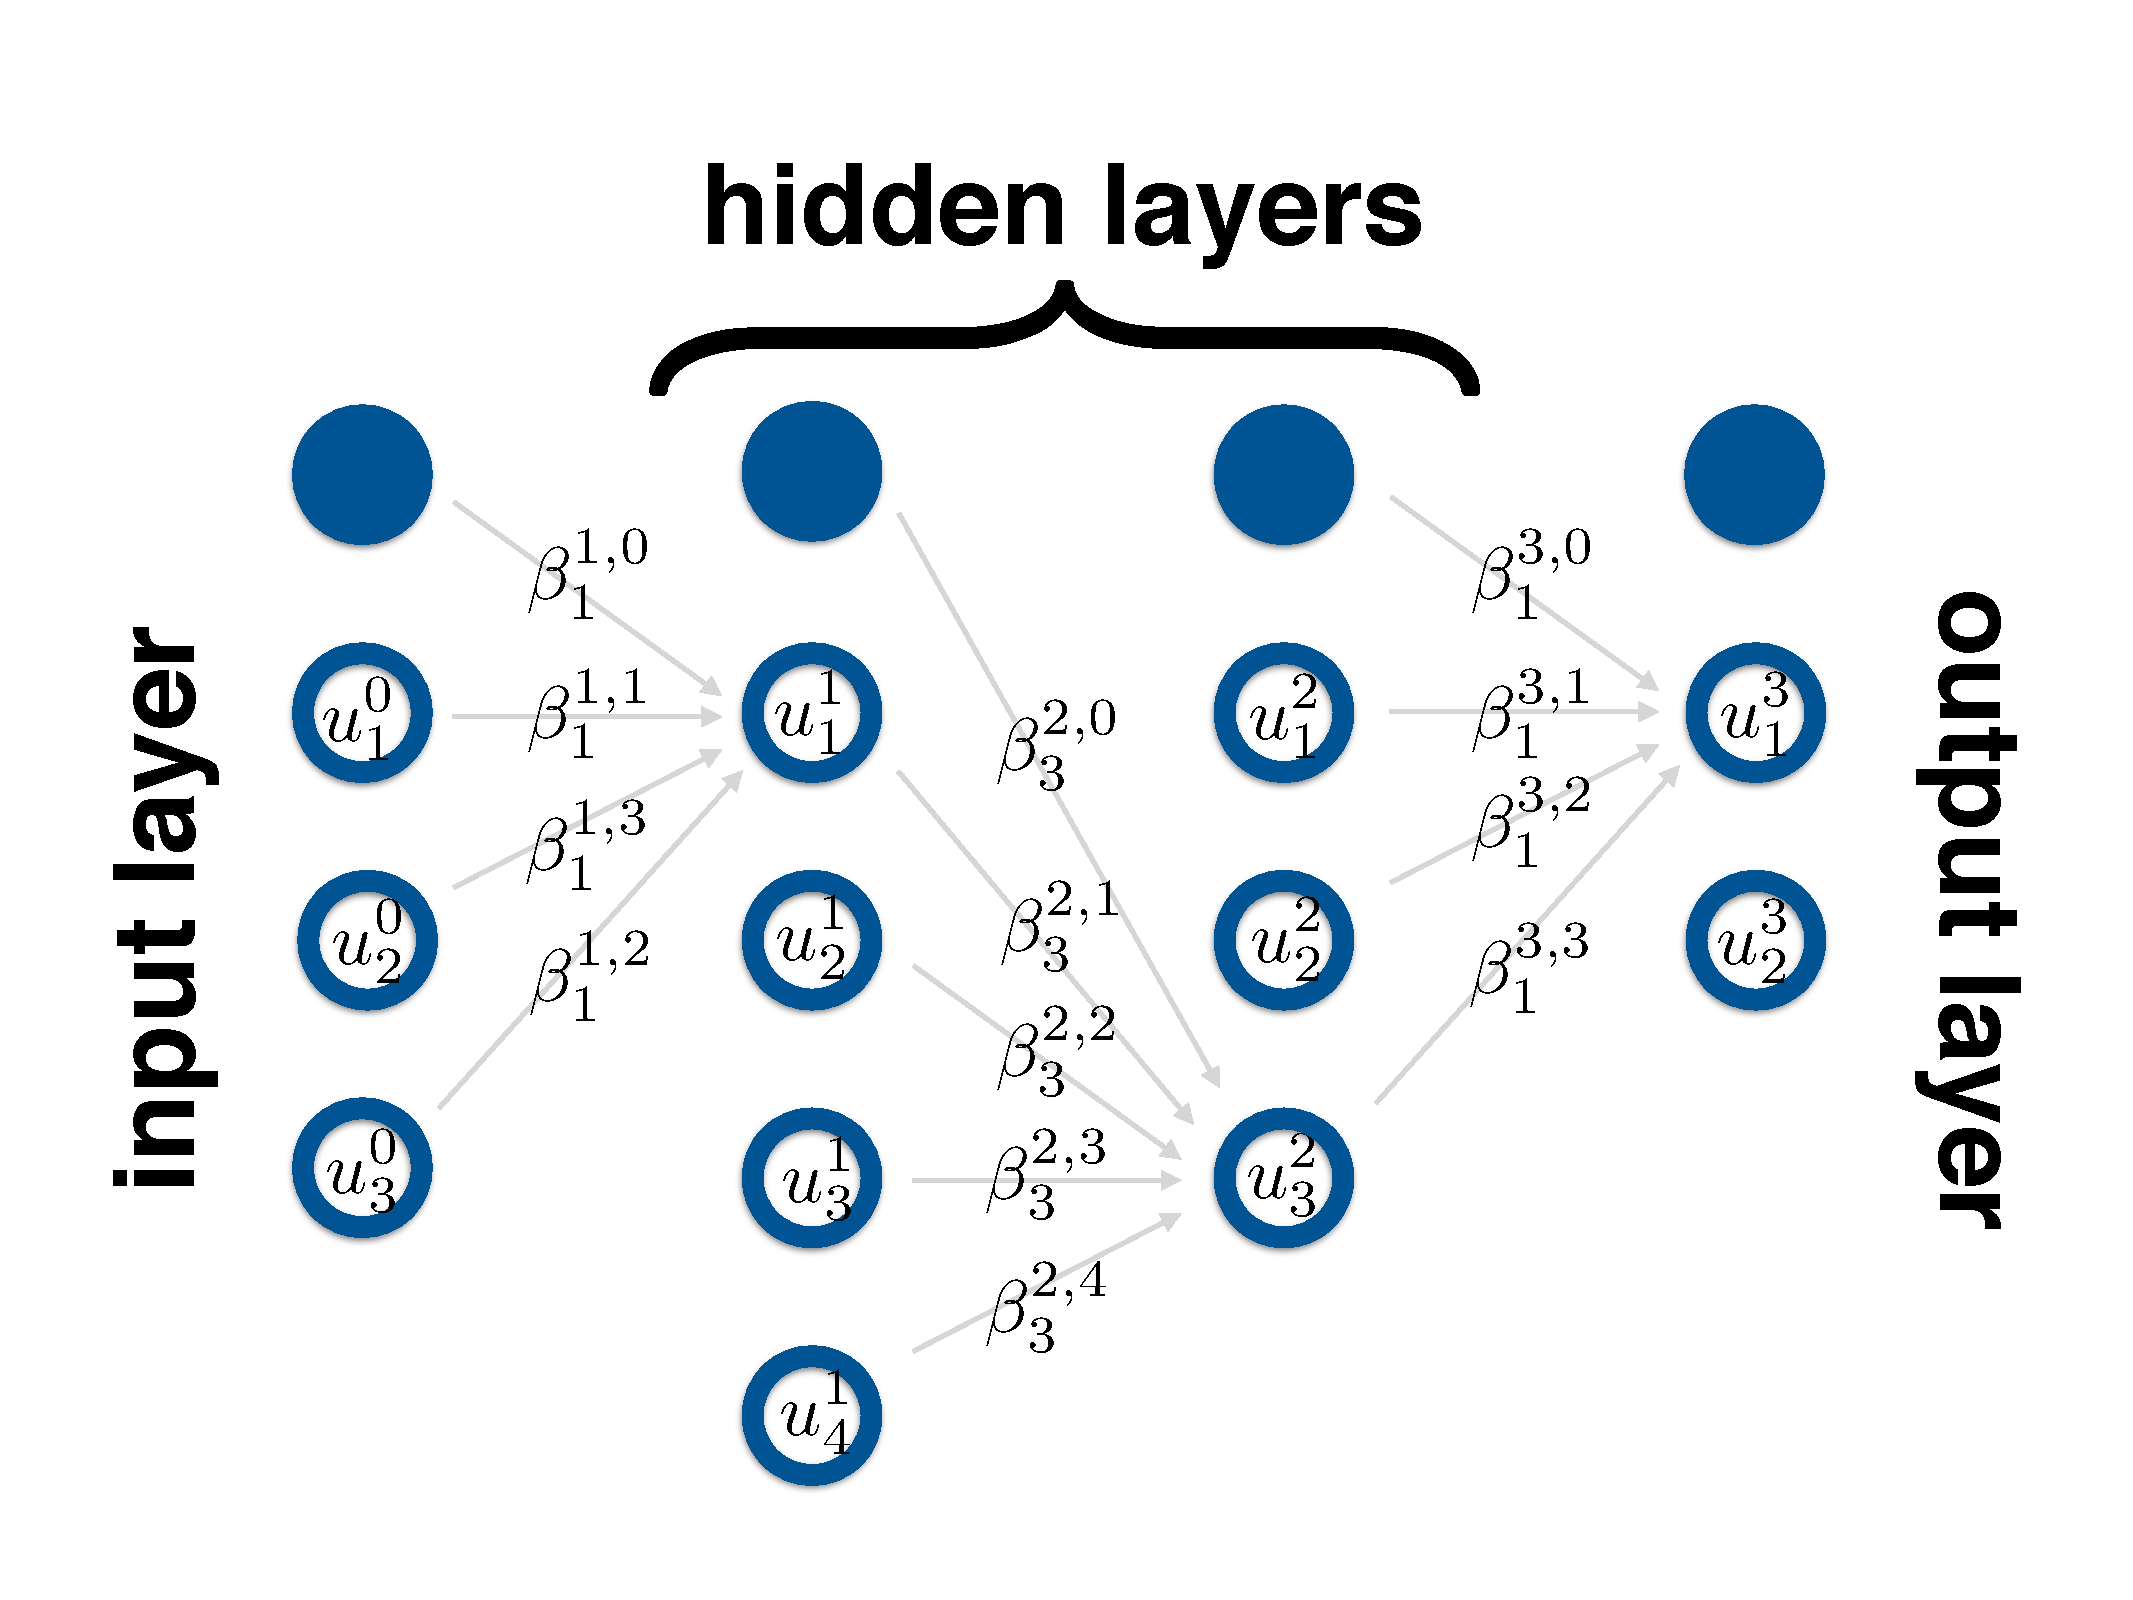
\includegraphics[width=.9\textwidth]{FFNN.pdf}
  \caption{Graphical representation of a Feed Forward Neural Network (FFNN). For a sake of clearness, only some connections are displayed.}
  \label{fig:FFNN}
\end{figure}

Despite the complex tasks that a FFNN can be used for, the math of a FFNN is extremely simple.
A FFNN can be interpreted as a function $f_H: \mathbb{R}^N \rightarrow \mathbb{R}^M$, where $N$ is the size of the input layer (i.e. its number of units, without counting the offset unit), and $M$ the size of the output layer.
The label $H$ represents the number of hidden layers of the FFNN.
Then, once that all the parameters $\beta$ are set, the FFNN output can be computed with the recursive formula:
\begin{equation}
  u^l_i = \actf( u^{l-1}_{k} \beta^{l,k}_{i}  )
\end{equation}
where $\actf: \mathbb{R} \rightarrow \mathbb{R}$ is a so-called \emph{activation function} and we have made use of the Einstein notation, for which repeated symbols on different levels imply a summation, e.g. $x_i^j y^i = \sum_i x_i^j y^i$.
The activation function is required to account for non-linear effects.
The FFNN library provides several well-known activation functions by default, but the user has the possibility to define and use its own, even though its storage on a file it is not supported (explained later).
These available activation functions are:
\begin{enumerate}
\item the \emph{logistic function}: $\logaf(x) \equiv \frac{1}{1+e^{-x}}$ \\
The current default for hidden and output units.
\item the \emph{tansig function}: $\tansaf(x) \equiv \frac{2}{1+e^{-2x}} - 1$ \\
Faster approximation to the regular tanh. Similar to logistic function, but with output in [-1,1].  
\item the \emph{gaussian}: $\gssaf(x) \equiv e^{-x^2}$ \\
Unlike normal activation functions it is symmetric around origin and not monotonic. Still there are use cases for it.
\item the \emph{sine function}: $\sinaf(x) \equiv sin(x)$ \\
Periodic activation function for special use cases.
\item the \emph{identity}: $\idaf(x) \equiv x$ \\
This function is linear and therefore should not be used for (all) hidden units.
\item the \emph{PReLU\footnote{\href{https://arxiv.org/abs/1502.01852}{arXiv:1502.01852}} function}: $\reluaf(x) \equiv 
\begin{cases}
  x & \text{if $x>0$} \\
  \alpha x & \text{if $x<=0$}
\end{cases}$ \\
The fixed hyper-parameter $\alpha$ defaults to 0. Due to their efficiency and because their gradient doesn't vanish, (Parametric) Rectified Linear Units are widely used in deep neural networks. However, the function is not differentiable at x=0 and has flat derivatives elsewhere. 
\item the \emph{SELU\footnote{\href{https://arxiv.org/abs/1706.02515}{arXiv:1706.02515}} function}: $\seluaf(x) \equiv \lambda 
\begin{cases}
  x & \text{if $x>0$} \\
  \alpha e^{x}- \alpha & \text{if $x<=0$}
\end{cases}$ \\
The Scaled Exponential Units (with two fixed hyper-parameters $\alpha$ and $\lambda$) solve some problems of ReLUs and can provide a self-normalizing network. But still they are not differentiable at x=0. 

\end{enumerate}
$\\$
The use of the FFNN library should be organised in four major steps:
\begin{enumerate}
\item generate the geometry of the FFNN;
\item connect the FFNN. This step will generate all the variational parameters $\beta$;
\item add substrates, required for computing the derivatives, if necessary;
\item set the input and propagate it through the FFNN in order to get the output.
\end{enumerate}

Now that the notation of the FFNN has been introduced, and we have briefly seen its structure and math, let us see the methods of this class:
\begin{itemize}
\item \verb+FeedForwardNeuralNetwork+: There are two possible constructors. The first one takes $3$ \verb+int+, which represents the size of the input, hidden (only one), and output layers. The user can change its shape later on. The values of $\beta$ will be set to some random values. The second constructor takes the path to a file where a FFNN has been stored;
\item \verb+getNHiddenLayers+: Return the number of hidden layers $H$;
\item \verb+getNLayers+: Return the total number of layers, i.e. $H+2$;
\item \verb+getLayerSize+: Return the size of the layer \verb+li+. Remember that $\verb+li+=0$ is reserved for the input layer and $\verb+li+=H+1$ for the output layer;
\item \verb+getLayerActivationFunction+: Return a pointer to the activation function used to obtain the layer \verb+li+. In the next section we will present the class \verb+ActivationFunctionInterface+;
\item \verb+getNBeta+: Return the total number of $\beta$;
\item \verb+getBeta+: Return the value of the $\beta^{l,p}_n$ corresponding to the \verb+ib+:
  $$
  {\verb+ib+} = {\verb+p+} + ({\verb+n+}-1) \, \verb+getLayerSize+({\verb+l+}-1) + \sum_{i=1}^{{\verb+l+}-1} \, \verb+getLayerSize+(i) \, \verb+getLayerSize+(i+1)
  $$
\item \verb+setBeta+: Set the value of a beta;
\item \verb+pushHiddenLayer+: Add an hidden layer of size \verb+size+ between the last hidden layer and the output layer. Notice that all the beta related to this layer will be set randomly;
\item \verb+popHiddenLayer+: Remove the last hidden layer (the one connected to the output layer);
\item \verb+setLayerSize+: Set the size of a Layer;
\item \verb+setGlobalActivationFunctions+: Set a global activation function for all the connections in the FFNN;
\item \verb+setLayerActivationFunction+: Set the activation function used to generate the layer \verb+li+;
\item \verb+addFirstDerivativeSubstrate+: Add a substrate that allows for the computation of the first derivatives of the FFNN in respect to the input, i.e. $\frac{\partial u^{H+1}_i}{\partial u^0_i}$;
\item \verb+addSecondDerivativeSubstrate+: Add a substrate that allows for the computation of the first derivatives of the FFNN in respect to the input, i.e. $\frac{\partial^2 u^{H+1}_i}{\partial {u^0_i}^2}$;
\item \verb+addVariationalFirstDerivativeSubstrate+: Add a substrate that allows for the computation of the first derivative of the FFNN in respect to the variational parameters $\beta$, i.e. $\frac{\partial u^{H+1}_i}{\partial \beta_{i}}$;
  % \item \verb+addLastHiddenLayerVariationalFirstDerivativeSubstrate+: Add a substrate that allows for the computation of the first variational derivatives of the $\beta$ in the last hidden layer only;
\item \verb+addCrossFirstDerivativeSubstrate+: Add a substrate that allows for the computation of the cross derivatives of the FFNN in respect to the input and the variational parameters $\beta$, i.e. $\frac{\partial^2 u^{H+1}_i}{\partial \beta_{j} \, \partial {u^0_i}}$;
\item \verb+addCrossSecondDerivativeSubstrate+: Add a substrate that allows for the computation of the cross second derivatives of the FFNN in respect to the input and the variational parameters $\beta$, i.e. $\frac{\partial^3 u^{H+1}_i}{\partial \beta_{j} \, \partial {u^0_i}^2}$;
\item \verb+connectFFNN+: Connect all the units in the FFNN. After this call it is possible to use the FFNN for computing quantities;
\item \verb+disconnectFFNN+: Disconnect all the units;
\item \verb+setInput+: Set the values of the units in the input layer. \verb+n+ is the size of the array \verb+in+, and if it does not suite the size of the input layer an error message will be thrown;
\item \verb+FFPropagate+: Compute the output values, including the derivatives if the substrates have been set accordingly;
\item \verb+getOutput+: Get the value of the unit \verb+i+ in the output layer;
\item \verb+getFirstDerivative+: Get the first derivative of the unit value $u^{H+1}_{\verb+i+}$ in respect to $u^0_{\verb+i1d+}$;
\item \verb+getSecondDerivative+: Get the second derivative of the unit value $u^{H+1}_{\verb+i+}$ in respect to $u^0_{\verb+i2d+}$;
\item \verb+getVariationalFirstDerivative+: Get the first derivative of the unit value $u^{H+1}_{\verb+i+}$ in respect to $\beta$ with $\verb+ib+ = \verb+iv1d+$. See \verb+getBeta+ for a definition of \verb+ib+;
\item \verb+getCrossFirstDerivative+: Get the cross derivative of the unit value $u^{H+1}_{\verb+i+}$ in respect to $u^0_{\verb+i1d+}$ and $\beta$ with $\verb+ib+ = \verb+iv1d+$;
\item \verb+getCrossSecondDerivative+: Get the second cross derivative of the unit value $u^{H+1}_{\verb+i+}$ in respect to $u^0_{\verb+i1d+}$ and $\beta$ with $\verb+ib+ = \verb+iv1d+$;
\item \verb+storeOnFile+: Store the FFNNon a file, making possible to retrieve it later on. If the activation functions have been customised, this procedure will not succeed.
\end{itemize}


\section{ActivationFunctionInterface} % (fold)
\label{sec:activationfunctioninterface}

\begin{lstlisting}
// #include "ActivationFunctionInterface.hpp"
class ActivationFunctionInterface
{
public:

      // allocate a new copy of this to returned ptr
      virtual ActivationFunctionInterface * getCopy() = 0;

      // return an unique identifier code
      virtual std::string getIdCode() = 0;

      // return the ideal input mean value (mu) and standard deviation (sigma)
      virtual double getIdealInputMu() = 0;
      virtual double getIdealInputSigma() = 0;

      // return the output mean value (mu) and standard deviation (sigma)
      // (pretending a flat distribution)
      virtual double getOutputMu() = 0;
      virtual double getOutputSigma() = 0;

      // compute the activation function value
      virtual double f(const double &) = 0;

      // first derivative of the activation function
      virtual double f1d(const double &) = 0;

      // second derivative of the activation function
      virtual double f2d(const double &) = 0;

      // third derivative of the activation function
      virtual double f3d(const double &) = 0;

      // calculate all derivatives together to save redundant calculations
      virtual void fad(const double &, const double &, const double &, const double &, const double &, const bool &, const bool &, const bool &);
};
\end{lstlisting}

The \verb+ActivationFunctionInterface+ is a pure virtual class, which can be used to generate customised activation functions to feed a FFNN.
It is necessary to provide implementations of all virtual methods except \verb+fad+ and highly recommended to provide \verb+fad+ (otherwise fad will use the other methods via virtual function calls -> slow).
As example we report the class for the logistic function:

\begin{lstlisting}
class LogisticActivationFunction: public ActivationFunctionInterface
{
   public:

      ActivationFunctionInterface * getCopy(){return new LogisticActivationFunction();}
      
      std::string getIdCode(){return "LGS";}

      // input should be in the rage [-5 : 5] -> mu=0   sigma=sqrt(3)
      double getIdealInputMu(){return 0.;}
      double getIdealInputSigma(){return 2.886751345948129;}

      // output is in the range [0 : 1] -> mu=0.5   sigma=1/(2*sqrt(3))
      double getOutputMu(){return 0.5;}
      double getOutputSigma(){return 0.288675134594813;}

      double f(const double &in)
      {
         return (1./(1.+exp(-in)));
      }

      double f1d(const double &in)
      {
         double f=this->f(in);
         return (f*(1.-f));
      }

      double f2d(const double &in)
      {
         double f=this->f(in);
         return (f*(1.-f)*(1.-2.*f));
      }

      double f3d(const double &in)
      {
         const double f = this->f(in);
         return f * (1. - f) * (1. - 6.*f + 6*f*f);
      }

      void fad(const double &in, double &v, double &v1d, double &v2d, double &v3d, const bool flag_d1 = false, const bool flag_d2 = false, const bool flag_d3 = false)
      {
         v = 1./(1.+exp(-in));

         if (flag_d1) {
            v1d = v * (1. - v);
            v2d = flag_d2 ? v1d * (1. - 2.*v) : 0.;
            v3d = flag_d3 ? v1d * (1. - 6.*v + 6.*v*v) : 0.;
         }
         else {
            v1d = 0.;
            v2d = flag_d2 ? v * (1. - v) * (1. - 2.*v) : 0.;
            v3d = flag_d3 ? v * (1. - v) * (1. - 6.*v + 6.*v*v) : 0.;
         }
      }
};

\end{lstlisting}

% section activationfunctioninterface (end)

\section{Training} % (fold)
\label{sec:training}

The library contains trainer classes for training a FFNN to match target data,
by the means of least squares fitting. All trainers derive from the virtual base class
\verb+NNTrainer+, which already contains the \verb+bestFit+ method to find the
best NN fit among several fits to target data.
Currently the only actual trainer implementation is the one using GSL nlinear
multifit, namely \verb+NNTrainerGSL+. This class provides the actual routine for
an individual fit, \verb+findFit+.
\\The trainer supports adding a L2 beta regularization residual term, controlled via
\verb+lambda_r+, and first/second derivative residual terms, controlled via
\verb+lambda_d1+ and \verb+lambda_d2+. In the latter case (if one of those
$\lambda$ is >0), the user has to
provide the respective derivative $\vec{y}_{d1_j}[]$, $\vec{y}_{d2_j}[]$ arrays with respect to all
input variables (index $j$) for every data point.
\\So concluding, the fully fledged residual \verb+R+ is computed as follows:
\begin{multline*}
  R^2 = \frac{1}{N} \sum_i^N  \left(\vec{f}(\vec{x}[i]) - \vec{y}[i]\right)^2 + \frac{1}{n_{\beta}} \sum_i^{n_{\beta}} \left( \lambda_r^2\ \beta_i^2 \right) \\
    + \frac{1}{N n_x} \sum_i^N \sum_j^{n_x} \left[ \lambda_{d1}^2\ (\partial_{x_j} \vec{f}(\vec{x}[i]) - \vec{y}_{d1_j}[i])^2  + \lambda_{d2}^2\ (\partial_{x_j}^2 \vec{f}(\vec{x}[i]) - \vec{y}_{d2_j}[i])^2 \right]
\end{multline*}
The design of the residual makes sure that it doesn't vary in magnitude with
respect to number of data point \verb+N+, input/output dimensions $n_x$,
$n_y$ or number of betas $n_{\beta}$.
\\\\How a complete code for NN training looks, you can see in the example 9.
If we leave out generating the data though, it comes down to the following:
\begin{lstlisting}
  #include "NNTrainerGSL.hpp"

  FeedFowardNeuralNetwork * ffnn =
      new FeedFowardNeuralNetwork(xndim+1, nhunits, yndim+1);
  ffnn->connectFFNN(); // only connect, don't add substrates
  ffnn->assignVariationalParameters(); // declare all betas to be variational parameters

  // create config and data structs
  // (for reference see respective header files)
  NNTrainingConfig tconfig =
      {lambda_r, lambda_d1, lambda_d2, maxn_steps, maxn_novali};
  NNTrainingData tdata =
      {ndata, ntraining, nvalidation, xndim, yndim, NULL, NULL, NULL, NULL, NULL};
  // instead of NULL you may pass existing allocations, but then don't use tdata.(de)allocate!  

  // allocate data arrays
  tdata.allocate(lambda_d1>0, lambda_d2>0)
  // if you provide deriv data in any case, just pass true

  // ... //
  // ... // fill tdata . x,y,w (and yd1/yd2 if you use derivs)
  // ... //

  // create trainer
  NNTrainerGSL * trainer = new NNTrainerGSL(tdata, tconfig);

  // (optional) setup ffnn's internal data normalization
  trainer->setNormalization(ffnn);

  // find a fit out of nfits with minimal testing residual
  trainer->bestFit(ffnn, nfits);

  // (optional) print output files along all axis
  trainer->printFitOutput(ffnn, lower_bound, upper_bound, npoints, flag_d1, flag_d2);

  tdata.deallocate();
  delete trainer;
  delete ffnn;

\end{lstlisting}
Afterwards, the \verb+ffnn+ will be in best fit configuration.
\\Make sure that you provide the necessary derivative data if you set
\verb+lambda_d1+ or \verb+lambda_d2+ greater than 0.
\\\\Also, it is important to understand the meaning of \verb+training+, \verb+validation+ and \verb+testing+
here:
\begin{itemize}
\item \verb+training+: The data that will be used by the least square solver itself.
  Especially the residual gradients will only be calculated from \verb+training+ data.
\item \verb+validation+: Every time the least square solver finds a new \verb+training+
  residual minimum, the residual of the \verb+validation+ data set will be calculated. If
  it didn't decrease (for too long, controlled by \verb+maxn_novali+), the
  fitting stops early.
\item \verb+testing+: When the individual fitting routine terminates (because
  \\\verb+maxn_steps+ reached or early stop), for the resulting fit the residual with
  respect to the \verb+testing+ data is calculated. Out of all fits, the fit with best
  \verb+testing+ residual is returned.
\end{itemize}
Note that \verb+validation+ can be disabled by setting \verb+nvalidation+ in the
\\\verb+NNTrainingData+ struct to 0 (this disables early stopping). \verb+testing+ however is disabled, if
\verb+ndata+ is equal to \verb+ntraining+ plus \verb+nvalidation+ (in this case
the training data set is used as replacement).
\\\\It is also possible to fine tune the GSL nlinear multifit algorithm by passing a
\verb+gsl_multifit_nlinear_parameters+ (see GSL docs) struct at trainer
creation:

\begin{lstlisting}
  gsl_multifit_nlinear_parameters your_gsl_parameters =
      gsl_multifit_nlinear_default_parameters();
  ... // tweak your gsl parameters
  NNTrainerGSL * trainer = new NNTrainerGSL(tdata, tconfig, your_gsl_parameters);
\end{lstlisting}
Finally, you can pass more arguments to \verb+bestFit+ to tweak the behavior:

\begin{lstlisting}
  trainer->bestFit(ffnn, nfits, resi_target, verbose, flag_smart_beta);
\end{lstlisting}
This will terminate the whole \verb+bestFit+ routine, if a \verb+testing+
residual below \verb+resi_target+ is found. Depending on int \verb+verbose+ (0,
1 or 2), it will print different levels of information. And if
\verb+flag_smart_beta+ is \verb+true+, it will use smart beta generation to
randomize betas before fitting. More about that in the next section. 

% section training (end)


\section{Smart Beta} % (fold)
\label{sec:smart_beta}

To understand this section, first read the pdf \verb+smart_initial_beta.pdf+ in
this folder. It should be noted that this feature is a bit experimental, so
double check that it actually works well for you.

It is possible to initialise the beta of a FFNN by doing the following:
\begin{lstlisting}
#include "SmartBetaGenerator.hpp"

FeedFowardNeuralNetwork * ffnn =
    new FeedFowardNeuralNetwork(4, 10, 2);
smart_beta::generateSmartBeta(ffnn);
\end{lstlisting}

For each unit we computed the desired $\mu_{\beta}$ and $\sigma_{\beta}$ using the formula reported in \verb+smart_initial_beta.pdf+, and sampled the beta accordingly.

To enforce the orthogonality we proceeded in the following way.
We sampled the first unit beta, a vector that we will now label as $v$. Then we sampled the second unit one, $u$, and applied the following modification:
\begin{equation}
   u \quad \rightarrow \quad u - \frac{\langle u, v \rangle}{\langle v, v \rangle} v     \label{eq:orthogonality}
\end{equation}
where $\langle u, v \rangle$ denotes the scalar product between $u$ and $v$.
This modification enforces the orthogonality.
We then multiply it by a scalar to make $u$ have the same norm as before the modification in Eq. \ref{eq:orthogonality}.
In case we sampled $u$ such that after the modification its norm is very small, we then sample it again.
We proceed in this way as long as possible. When we have enough beta to form a complete basis set, we stop applying the orthogonality procedure and we sample them randomly again.

% section smart_beta (end)


\section{Serializable Components} % (fold)
\label{sec:serializablecomponents}
All classes deriving from SerializableComponent (i.e. all components of our
network) support serialization of their restorable configuration (e.g. pointers
to other runtime objects usually can't be restored) into simple strings, by a
code system. It is explained in detail in
the StringCodeUtilities.hpp header file and the examples, but will quickly be
illustrated here.
\\Consider an output unit (type id \verb+OUT+) of our neural network. It has two simple parameters
\verb+shift+ and \verb+scale+ and itself two \verb+SerializableComponent+ members, the
feeder \verb+RAY+ and the activation function \verb+LGS+ (default). If we
assume the ray has no beta parameters set yet, the full serialized object string (treeCode)
looks like:
\begin{verbatim}
string treeCode = "OUT ( shift 0.0 , scale 1.0 ) { RAY , LGS }"
\end{verbatim}
If \verb+RAY+ and \verb+LGS+ had own parameters or members, they would be appended after their
identifier, enclosed in () or \{\} brackets, respectively.
\\\\NOTE: Because the system relies on the spacing between every token, the
spaces must not be neglected. Also a parameter value of string type may not
contain any spaces, commas or brackets of kind () or \{\}.

% section serializablecomponents (end)


\printindex

\end{document}
